\documentclass{article}

% if you need to pass options to natbib, use, e.g.:
% \PassOptionsToPackage{numbers, compress}{natbib}
% before loading nips_2016
%
% to avoid loading the natbib package, add option nonatbib:
% \usepackage[nonatbib]{nips_2016}

\usepackage[final]{nips_2016}

% to compile a camera-ready version, add the [final] option, e.g.:
% \usepackage[final]{nips_2016}

\usepackage[utf8]{inputenc} % allow utf-8 input
\usepackage[T1]{fontenc}    % use 8-bit T1 fonts
\usepackage{hyperref}       % hyperlinks
\usepackage{url}            % simple URL typesetting
\usepackage{booktabs}       % professional-quality tables
\usepackage{amsfonts}       % blackboard math symbols
\usepackage{nicefrac}       % compact symbols for 1/2, etc.
\usepackage{microtype}      % microtypography
\usepackage{mathtools}
\usepackage{amssymb}
\usepackage{amsthm}
\usepackage{amsmath}
\usepackage{verbatim}  
\usepackage{enumerate}
\usepackage{fancyvrb}
\usepackage{bm}
\usepackage{bbm}
\usepackage{dsfont}
\usepackage{hyperref}
\usepackage[pdftex]{graphicx}
\DeclareMathOperator*{\argmin}{arg\,min}
\DeclareMathOperator*{\argmax}{arg\,max}
\def\real{\mathbb{R}}
\def\cS{{\cal S}}
\def\cG{{\cal G}}
\def\cb{{\cal B}}
\def\ca{{\cal A}}
\def\cR{{\cal R}} 
\def\cep{{\cal \varepsilon}}
\newtheorem{lemma}{Lemma}[section]
\newtheorem{proposition}{Proposition}[section]
\newtheorem{theorem}{Theorem}[section]
\newtheorem{remark}{Remark}[section]
\newtheorem{definition}{Definition}[section]
\newtheorem{property}{Property}[section]

\title{Literature Review: GAP Safe Screening Rules for Sparse-Group Lasso}

% The \author macro works with any number of authors. There are two
% commands used to separate the names and addresses of multiple
% authors: \And and \AND.
%
% Using \And between authors leaves it to LaTeX to determine where to
% break the lines. Using \AND forces a line break at that point. So,
% if LaTeX puts 3 of 4 authors names on the first line, and the last
% on the second line, try using \AND instead of \And before the third
% author name.

\author{
  Gang Cheng
  %\thanks{Use footnote for providing further
  %  information about author (webpage, alternative
   % address)---\emph{not} for acknowledging funding agencies.} 
    \\
  Department of Statistics\\
  University of Washington\\
  Seattle, WA 98195 \\
  \texttt{gangc@uw.edu} \\
  %% examples of more authors
  %% \And
  %% Coauthor \\
  %% Affiliation \\
  %% Address \\
  %% \texttt{email} \\
  %% \AND
  %% Coauthor \\
  %% Affiliation \\
  %% Address \\
  %% \texttt{email} \\
  %% \And
  %% Coauthor \\
  %% Affiliation \\
  %% Address \\
  %% \texttt{email} \\
  %% \And
  %% Coauthor \\
  %% Affiliation \\
  %% Address \\
  %% \texttt{email} \\
}

\begin{document}
% \nipsfinalcopy is no longer used

\maketitle

\begin{abstract}
In this paper review, I gave a summary of the paper: GAP Safe Screening Rules for sparse-group lasso. I also provided a few proofs for problems that I am not so familiar with, like the dual formulation of the penalized regression problem, the group soft-thresholding operator and the block-wise Lipschitz constant.  I also run two numerical experiments for the algorithm mentioned in the original paper. 
\end{abstract}

\section{Introduction}

This paper is mainly about solving the problem of sparse-group lasso, which could be framed in the following penalized regression form
\begin{align}
\hat{\beta}^{(\lambda,\Omega)} \in \argmin\limits_{\beta \in \real^p} \frac{1}{2}\|y - X\beta\|_2 + \lambda \Omega(\beta) := P_{\lambda,\Omega}(\beta)
\end{align}
where $\lambda > 0$. Here, $\Omega(\lambda)$ is the sparse-group lasso norm where we defined in the following. 

\paragraph{Notation} For any integer $d \in \mathbb{N}$, we denote by $[d]$ the set $\{1,\ldots,d\}$. Response $y \in \real^n$ and the design matrix $X = [X_1,\ldots,X_p] \in \real^{n \times p}$ has p features. Here, we assume our parameter $\beta = (\beta_1,\ldots,\beta_p)$ admits a group structure. A group of features is a subset $g \subset [p]$ and $n_g$ is its cardinality. The set of groups is denoted by $\cal{G}$  We denote by $\beta_g$ the vector in $\real^{n_g}$ which is the restriction of $\beta$ to the indexes in g. We write $[\beta_g]_j$ the j-th coordinate of $\beta_g$. We also use the notation $X_g \in \real^{n \times n_g}$ for the sub-matrix of X containing only features in group g;  similarly defined $[X_g]_j$ as the j-th column of $X_g$. The soft-thresholding operator,$\cS_{\tau}$  is defined for any $x \in \real^d$ by $[\cS_{\tau}( x )]_j = \text{sign}(x_j)(|x_j| - \tau)_{+}$ and the group soft-thresholding operator is $\cS^{gp}_{\tau}(x) = (1 - \tau/\|x\|)_{+}x$.

Now we can define the sparse-group lasso norm. Let $\tau \in [0,1], w =(w_g)_{g \in \cal{G}}$  with $w_g \geq 0$ for all $g \in \cal{G}$. Then we have 
\begin{align}
\Omega(\beta): = \tau \|\beta\|_1 + (1-\tau)\sum_{g \in \cal{G}} \|\beta_g\|
\end{align}
Further the case where $w_g = 0$ for some $g \in \cal{G}$ together with $\tau = 0$ is excluded.

Thus,  we have  $f(\beta) = \frac{1}{2}\|y-X\beta\|^2$, which is simply the empirical error.  

\section{Sparse-Group lasso}

\subsection{Dual formulation}

One important point in the paper is to employ the dual formulation of the sparse-group lasso problem.  Below is the dual formulation for the primal problem (1). 
\begin{align}
\hat{\theta}^{(\lambda,\Omega)} = \argmax\limits_{\theta \in \Delta_{X,\Omega}} \frac{1}{2} \|y\|^2 - \frac{\lambda^2}{2}\|\theta - \frac{y}{\lambda}\|^2 := D_{\lambda}(\theta)
\end{align}
where $\Delta_{X,\Omega} = \{\theta \in \real^n : \Omega^D(X^T\theta) \leq 1\}$. 
\begin{proof} ~\newline
Rewrite problem (1) in the following form 
\begin{equation}
\begin{aligned}
& \hat{\beta}^{(\lambda,\Omega)} \in \argmin\limits_{\beta \in \real^p} \frac{1}{2}\|y - z\|^22 + \lambda \Omega(\beta) \\
& \text{s.t. } z = X\beta 
\end{aligned}
\end{equation}
Its dual is 
\begin{align}
L(\gamma) = \argmin\limits_{z,\beta} \frac{1}{2}\|y-z\|^2 + \lambda \Omega(\beta) + \gamma^T(z-X\beta)
\end{align}
Setting the subgradient of equation (5) to be zero give
\begin{equation}
\begin{aligned}
& \gamma = y - z \\ 
&  X^T \gamma \in \lambda \partial \Omega(\beta)
\end{aligned}
\end{equation}
Then we could obtain the dual formulation being
\begin{align}
-\frac{1}{2}\|\gamma\|^2 + \gamma^Ty
\end{align}
with $\Omega^D(X^T\gamma) \leq \lambda$.  Further if we let $\gamma = \theta \lambda$, we could get dual formulation (3) with the following two equations from (6):
\begin{align}
\lambda \hat{\theta}^{(\lambda,\Omega)} = y - X \hat{\beta}^{(\lambda,\Omega)} \quad \textbf{(link-equation)} \\
X^T \hat{\theta}^{(\lambda,\Omega)} \in \partial \Omega(\hat{\beta}^{(\lambda,\Omega)} \ \textbf{(sub-differential inclusion)}
\end{align}
\end{proof}



\subsection{Sparsity pattern}

The sparse-group lasso norm is $\Omega(\beta) = \tau \|\beta\|_1 + (1-\tau)\sum_{g \in \cal{G}} w_g \|\beta_g\|$.  The  $l_1$ norm is for sparsity and the $l_{1,2}$ norm is for group sparsity. Thus, this norm is enforcing sparsity and group-sparsity at the same time.  We will recover the LASSO if $\tau = 1$, and the group lasso if $\tau = 0$. 


\subsection{Proximal operator for sparse-group lasso}



For sparse-group lasso norm, we have that $f(\beta) = \frac{1}{2} \|y - X\beta\|^2$. Thus, we have that $\nabla f(\beta) = -X^T(y-X\beta)$. 
For simplicity, assuming that $\cG = \{g_1,\ldots,g_m\}$, which means that we have m groups in total. According to Jenatton et.al 2010, we know that the proximal operator of sparse-group lasso norm could be decomposed[2,3] as following:
\begin{equation}
\begin{aligned}
\text{Prox}_{\Omega(\beta)}(v) & = \text{Prox}_{(1-\tau)\sum_{g \in \cal{G}}w_g\|\beta_g\|}(\text{Prox}_{\tau \|\beta\|_1}(v)) \\
& = \text{Prox}_{(1-\tau)\sum_{g \in \cal{G}}w_g\|\beta_g\|}(S_{\tau}(v))\\
& = \text{Prox}_{(1-\tau)\sum_{\substack{g \in \cal{G} \\ g \neq g_1}}w_g\|\beta_g\|}\left[\text{Prox}_{(1-\tau)w_{g_1}\|\beta_{g_1}\|}(S_{\tau}(v))\right]\\
& = \text{Prox}_{(1-\tau)\sum_{\substack{g \in \cal{G} \\ g \neq g_1}}w_g\|\beta_g\|}\left[\cS^{gp}_{(1-\tau)w_{g_1}}(S_{\tau}(v))\right]\\
& = \cS^{gp}_{(1-\tau)w_{g_m}} \circ \ldots \circ \cS^{gp}_{(1-\tau)w_{g_1}}(S_{\tau}(v))\\
\end{aligned}
\end{equation}
Thus, the proximal operator of sparse-group lasso is computed by applying soft-thresholding operator first and then applying group-thresholding operator for all the groups.  This motivates the use of block coordinate descent algorithm.  I will skip the proof for soft-thresholding and give a proof for group-thresholding:
\begin{proof} ~\newline
 Assuming we are applying proximal operator on group $g$, 
$$
\text{Prox}_{(1-\tau)w_g\|\beta_g\|}(x) = \argmin\limits_{\beta} (1-\tau)w_g \|\beta_g\| + \frac{1}{2}\|x - \beta\|^2
$$
Since we are only focusing on $\beta_g$, for the rest parameters, we could simply set $\beta_{-g} = x_{-g}$.
Then the problem becomes
$$
\argmin\limits_{\beta_g} (1-\tau)w_g\|\beta_g\| + \frac{1}{2}\|x_g - \beta_g\|^2
$$
Let's take the subgradient of the above formula, then we have 
$$
0 \in (1-\tau)w_g \partial  \|\hat{\beta}_g\| - x_g + \hat{\beta}_g 
$$
Thus, we should have that 
\begin{align}
\hat{\beta}_g = x_g - (1-\tau)w_g \partial \|\hat{\beta}_g\|
\end{align}
if $\hat{\beta}_g = 0$, we have $\partial \|\hat{\beta}_g\| = \frac{1}{(1-\tau)w_g}x_g$, which should satisfy the condition that $\|\partial \|\hat{\beta}_g\| \| \leq 1 \rightarrow \frac{(1-\tau)w_g}{\|x_g\|} \geq 1$. 

if $\hat{\beta}_g \neq 0$, then we have $\partial \|\hat{\beta}_g\| = \frac{\hat{\beta}_g}{\|\hat{\beta}_g\|}$ and if we take this back to equation (11), we have 
$$
\hat{\beta}_g(1 + (1-\tau)w_g/\|\hat{\beta}_g\|) = x_g
$$
which means that $\hat{\beta}_g = \gamma x_g$ for some constant $\gamma > 0$.  If we set $\hat{\beta}_g = \gamma x_g$ in equation (11), then we can get 
$$
\hat{\beta}_g = x_g - (1-\tau)w_g \frac{x_g}{\|x_g\|} = x_g\left[1 - \frac{(1-\tau)w_g}{\|x_g\|}\right]
$$
with $\frac{(1-\tau)w_g}{\|x_g\|} < 1$.  Then combined with the case $\hat{\beta}_g = 0$, we have that 
$$
\hat{\beta}_g = (1 - (1-\tau)w_g/\|x_g\|)_{+} x_g = \cS^{gp}_{(1-\tau)w_g}(x_g)
$$
\end{proof}

Naturally, (10) leads to the following block coordinate descent algorithm:
at iteration $l$, we choose (cyclically) a group $g$ and the next iterate $\beta^{l+1}$ is defined as $\beta_{g'}^{l+1} = \beta_{g'}^l$ if $g' \neq g$ and otherwise $\beta_g^{l+1} = \cS^{gp}_{(1-\tau)w_g\alpha_g}(\cS_{\tau \alpha_g}(\beta_g^l - \nabla_g f(\beta^l)/L_g))$ where $L_g$ is the block-wise Lipschitz constant for $f(\beta) = 1/2\|y- X\beta\|^2$ and $\alpha_g = \lambda/L_g$.  Here, an appropriate $L_g$ would be $\|X_g\|_2^2$, the square of the spectral norm of $X_g$.  A proof would be following:
\begin{proof} ~\newline
Consider only the parameter only in group $g$ and the problem become 
$$
f'(\beta_g) = \frac{1}{2}\|Y - X_g \beta_g\|^2
$$
It's hessian is $\nabla \nabla f'(\beta_g) = X_g^T X_g$. Thus an appropriate Lipschitz constant would be $\lambda_{\text{max}}(X_g^T X_g)$, the maximum eigenvalue of $X_g^T X_g$, which is simply $\|X_g\|_2^2$.  
\end{proof}




\section{GAP safe rule for the sparse group lasso}

This section is mostly from the original paper[1], which below I quote sentences without reference. 
The main idea of the paper is to reduce the computational burden of solving sparsity problems in high dimension. The screening rules exploit the known sparsity of the solution to reduce the computation. They compute some tests on dual feasible points to eliminate primal variables whose coefficients are guaranteed to be zero. However, for sparse-group lasso, the computation of a feasible dual point is quite challenging. Thus, the authors propose an efficient computation of the associated dual norm.  Being able to efficiently compute the dual norm, they proposed \textbf{GAP SAFE} screening rules for the sparse-group lasso that combines sequential rules(\textit{i.e}, rules that perform screening thanks to solutions obtained for a previously processed parameter) and dynamic rules(\textit{i.e}, rules that perform screening as the algorithm proceeds) in a unified way[1]. 

The main contributions in this paper are in two ways.  First, they introduced the first safe screening rules for the sparse-group lasso problem. Second, they linked the sparse-group lasso penalties to the $\epsilon$-norm, which allows to provide a new algorithm to efficiently compute the required dual norm.

\subsection{Description of the screening rules}
Sparse-group lasso benefits from two levels of screening: the safe rules can detect both group-wise zeros in the vector $\hat{\beta}^{\lambda,\Omega}$ and coordinate-wise zeros in the remaining groups. 

\begin{proposition}[Theoretical screening rules]
The two levels of screening rules for the Sparse-Group Lasso are:\\
\textbf{Feature level screening:}
$$
\forall j \in g, |X_j^T \hat{\theta}^{(\lambda,\tau,w)}| < \tau \rightarrow \hat{\beta}_j^{(\lambda,\tau,w)} = 0
$$
\textbf{Group level screening:}
$$
\forall g \in \cG, \|\cS_{\tau}(X_g^T \hat{\theta}^{(\lambda,\tau,w)})\|  < (1-\tau)w_g \rightarrow \hat{\beta}_g^{(\lambda,\tau,w)} = 0
$$
\end{proposition}
This theoretical screening rules involve the unknown $\hat{\theta}^{(\lambda,\tau,w)}$. Thus to obtain useful screening rules one need a \textbf{safe region}, a set containing the optimal dual solution $\hat{\theta}^{(\lambda,\Omega)}$.  They chose a ball $\cb( \theta_c, r)$ with radius r and centered at $\theta_c$ as a safe region, call it a safe sphere. The safe rules for the Sparse-Group lasso work as follows: for any group $g$ in $\cG$ and any safe sphere $\cb(\theta_c,r)$.
\begin{align}
& \textbf{Group level safe screening:} \max\limits_{\theta \in \cb(\theta_c, r)} \|S_{\tau} (X_g^T \theta)\| < (1-\tau) w_g \rightarrow \hat{\beta}_g^{(\lambda,\tau,w)} = 0 \\
& \textbf{Feature level screening:} \forall j \in g, \max\limits_{\theta \in \cb(\theta_c,r)} |X_j^T \theta| < \tau \rightarrow \hat{\beta}_j^{(\lambda,\tau,w)} = 0
\end{align}
Thusl, naturally a safe sphere is more useful with $r$ smaller and $\theta_c$ closer to $\hat{\theta}^{\lambda,\tau,w}$.  Further to employ this screening rule, we need to upper bound on $\max\limits_{\theta \in \cb(\theta_c, r)} \|S_{\tau} (X_g^T \theta)\|$ and $\max\limits_{\theta \in \cb(\theta_c,r)} |X_j^T \theta|$, which is the following:
\begin{proposition}
For all groups $g \in \cG$ and $j \in g$, \\
\begin{align}
\max\limits_{\theta \in \cb(\theta_c,r)} |X_j^T \theta| \leq |X_j^T \theta_c| + r \|X_j\| 
\end{align}
and 
\begin{align}
\max\limits_{\theta \in \cb(\theta_c, r)} \|S_{\tau} (X_g^T \theta)\| \leq {\cal T}_g := \begin{cases} \|\cS_{\tau} (X_g^T \theta_c)\| + r\|X_g\| & if \|X_g^T \theta_c\|_{\infty} > \tau, \\ 
(\|X_g^T \theta_c\|_{\infty} + r\|X_g\| - \tau)_{+}  & \text{otherwise} \end{cases}
\end{align}
\end{proposition}

These two upper bounds combined with the above safe screening rules, we have that 
\begin{theorem}[Safe rules for Sparse-group lasso]. 
Using ${\cal T}_g$ defined in equation (15), we can state the following safe screening rules:
\begin{align}
& \textbf{Group level safe screening:} \forall g \in {\cal T}_g  < (1-\tau) w_g \rightarrow \hat{\beta}_g^{(\lambda,\tau,w)} = 0 \\
& \textbf{Feature level screening:} \forall j \in g, |X_j^T \theta_c| + r\|X_j\| < \tau \rightarrow \hat{\beta}_j^{(\lambda,\tau,w)} = 0
\end{align}
\end{theorem}

\subsection{Computation of gap safe sphere}

The computation of the gap safe sphere comprises of the computation of the radius and the computation of the center, which is a dual feasible point. 

\subsubsection{Computation of the center}
The authors leverage the primal/dual link-equation(8) to dynamically construct a dual point based on a current approximation $\beta_k$ of $\hat{\beta}^{(\lambda,\tau,w)}$. Note that $\beta_k$ is the primal value at iteration $k$ obtained by an iterative algorithm. Starting from a current residual $\rho_k = y - X\beta_k$, one can create a dual feasible point by choosing for all $k \in \mathbb{N}$:
\begin{align}
\theta_k = \frac{\rho_k}{\max(\lambda,\Omega^D_{\tau,w}(X^T \rho_k))}
\end{align}
We refer to $\cb(\theta_k, r_{\lambda,\tau}(\beta_k,\theta_k))$ as GAP safe spheres.  It's easy to verify that $\theta_k$ is indeed a dual feasible point since $\Omega^D_{\tau,w}(X^T \theta_k) = \frac{\Omega^D_{\tau,w}(X^T \rho_k)}{\max(\lambda,\Omega^D_{\tau,w}(X^T \rho_k)} \leq 1$.

\subsubsection{Computation of the radius}
With a dual feasible point $\theta \in \Delta_{X,\Omega}$ and any $\beta \in \real^p$, one has $\hat{\theta}^{(\lambda,\tau,w)} \in \cb(\theta,r_{\lambda,\tau}(\beta,\theta))$, for 
$$
r_{\lambda,\tau}(\beta,\theta) = \sqrt{\frac{2(P_{\lambda,\tau,w}(\beta) - D_{\lambda}(\theta)}{\lambda^2}}
$$
\begin{proof} ~\newline
By weak duality, $\forall \beta \in \real^p$, $D_{\lambda}(\hat{\theta}^{(\lambda,\tau,w)} \leq P_{\lambda,\tau,w}(\beta)$. Then since the dual formualtion is $\lambda^2$-strongly concave, we have 
$$
\forall (\theta,\theta') \in \Delta_{X,\Omega} \times \Delta_{X,\Omega}, \quad D_{\lambda}(\theta) \leq D_{\lambda}(\theta') + \nabla D_{\lambda}(\theta')^T (\theta - \theta') - \frac{\lambda^2}{2}\|\theta - \theta'\|^2
$$
Set $\theta' = \hat{\theta}^{(\lambda,\tau,w)}$, we should have that 
$$
\Delta D_{\lambda}( \hat{\theta}^{(\lambda,\tau,w)})(\theta -  \hat{\theta}^{(\lambda,\tau,w)}) \leq 0
$$
Since $\hat{\theta}^{(\lambda,\tau,w)}$ maximize the $D_{\lambda}(\theta)$. Then, we have that 
\begin{align}
\frac{\lambda^2}{2}\|\theta -  \hat{\theta}^{(\lambda,\tau,w)}\|^2 &\leq D_{\lambda}(\hat{\theta}^{(\lambda,\tau,w)}) - D_{\lambda}(\theta) \\
& \leq P_{\lambda,\tau,w}(\beta) - D_{\lambda}(\theta)
\end{align}
\end{proof}

Then the only problem left now is to calculate the dual norm $\Omega^D$. The author proposed to use $\epsilon_norm$, a norm that can be efficiently computed, to calculate it.  I will skip the part related to $\epsilon$-norm here. 

\subsection{Convergence of the active set}
This section proves that the sequence of dual feasible points obtained from (18) converges to the dual solution $\hat{\theta}^{(\lambda,\Omega)}$ if $\beta_k$ converges to an optimal solution $\hat{\beta}^{(\lambda,\Omega)}$.  Further, we know that with strong duality, $P_{\lambda,\tau,w}(\hat{\beta}^{(\lambda,\tau,w)}) = D_{\lambda}(\hat{\theta}^{(\lambda,\tau,w)}$. Thus, we have $\lim_{k \to \infty} r_{\lambda,\tau}(\beta_k,\theta_k) = 0$.

\begin{proposition}
if $\lim_{k \to \infty} \beta_k = \hat{\beta}^{(\lambda,\tau,w)}$, then $\lim_{k to \infty} \theta_k = \hat{\theta}^{(\lambda,\tau,w)}$. 
\end{proposition}
\begin{proof}
Let $\alpha_k  = \max(\lambda, \Omega^D_{\tau,w}(X^T \rho_k))$ and $\rho_k = y - X\beta_k$. We have
\begin{align*}
\|\theta_k - \hat{\theta}^{(\lambda,\tau,w)}\| & = \Big\|\frac{1}{\alpha_k}(y - X\beta_k) - \frac{1}{\lambda}(y - X\hat{\beta}^{(\lambda,\tau,w)})\Big \| \\ 
& = \Big \| \left(\frac{1}{\alpha_k} - \frac{1}{\lambda}\right)(y - X \beta_k) + \frac{(X \hat{\beta}^{(\lambda,\tau,w)} - X\beta_k)}{\lambda} \Big \| \\
&  \leq \Big | \frac{1}{\alpha_k} - \frac{1}{\lambda} \Big | \|y - X\beta_k\| + \Big \| \frac{(X \hat{\beta}^{(\lambda,\tau,w)} - X\beta_k)}{\lambda} \Big \|. 
\end{align*}
Here if $\beta_k \to \hat{\beta}^{(\lambda,\tau,w)}$, then $\alpha_k \to \max(\lambda,\Omega^D(\tau,w) (X^T(y - X\hat{\beta}^{(\lambda,\tau,w)})) = \max(\lambda,\lambda \Omega^D_{\tau,w}(X^T \hat{\theta}^{(\lambda,\tau,w)})) = \lambda$.  Since $\Omega^D_{\tau,w}(X^T\hat{\theta}^{(\lambda,\tau,w)}) \leq 1$. Hence, both terms in the previous inequality converge to zero. 
\end{proof}

Next, we define two levels of active sets, 
\begin{align*}
& \ca_{\text{groups}}(\cR): = \left\{ g \in \cG, \ \max\limits_{\theta \in \cR} \|\cS_{\tau}(X_g^T\theta)\| \geq (1-\tau) w_g \right\} \\
& \ca_{\text{features}}(\cR) := \bigcup\limits_{g \in \ca_{\text{groups}}(\cR)} \left\{ j \in g: \max_{\theta \in \cR}\|X_j^T \theta| \geq \tau \right\}.
\end{align*}
if one considers sequence of converging regions, the next proposition states that we can identify, in finite time, the optimal active sets defined as follows:
\begin{align*}
& \cep_{\text{groups}}: = \left\{ g \in \cG, \  \|\cS_{\tau}(X_g^T\hat{\theta}^{(\lambda,\tau,w)})\| \geq (1-\tau) w_g \right\} \\
& \cep_{\text{features}} := \bigcup\limits_{g \in \cep_{\text{groups}}} \left\{ j \in g: \|X_j^T \hat{\theta}^{(\lambda,\tau,w)}| \geq \tau \right\}.
\end{align*}
\textbf{In the original paper, the authors defined $\cep_{\text{groups}}: = \left\{ g \in \cG, \  \|\cS_{\tau}(X_g^T\hat{\theta}^{(\lambda,\tau,w)})\| = (1-\tau) w_g \right\}$,  I suppose this should be typo}.

\vspace{2em}
\begin{proposition}
Let $(\cR_k)_{k in \mathbb{N}}$ be a sequence of safe regions whose diameters converge to 0. Then $\lim\limits_{k \to \infty} \ca_{\text{groups}}(\cR_k) = \cep_{\text{groups}}$ and $\lim\limits_{k \to \infty}\ca_{\text{features}}(\cR_k) = \cep_{\text{features}}$
\end{proposition}
\begin{proof} ~\newline
First, it's easy to prove that $\forall k \in \mathbb{N}$, $\cep_{groups} \subset \ca_{\text{groups}}(\cR_k)$. The idea is that if $\|\cS_{\tau}(X_g^T \hat{\theta}^{(\lambda,\tau,w)})\| = (1-\tau)w_g$, then we should that $\max\limits_{\theta \in \cR}\|\cS_{\tau}(X_g^T \theta)\| \geq \|\cS_{\tau}(X_g^T \hat{\theta}^{(\lambda,\tau,w)})\| = (1-\tau)w_g$ since $\hat{\theta}^{(\lambda,\tau,w)} \in \cR_k$.  Thus, if $g \in \cep_{\text{groups}}$, then $g \in \ca_{\text{groups}}$.

For the other side, since we already have that $\lim_{k \to \infty} r_{\lambda,\tau}(\beta_k,\theta_k) = 0$, thus, for $\forall \epsilon >0$, there $\exists k_0 \in \mathbb{N}$, such that $\forall k \geq k_0$, $\forall \theta \in \cR_k$, we have $\|\theta - \hat{\theta}^{(\lambda,\tau,w)}\| \leq \epsilon$.  \\ 
Then for $\forall g \notin \cep_{\text{groups}}$,  $\|\cS_{\tau}(X_g^T \theta)\| \leq \| \cS_{\tau}(X_g^T \theta) - \cS_{\tau}(X_g^T \hat{\theta}^{(\lambda,\tau,w)})\| + \|\cS_{\tau}(X_g^T \hat{\theta}^{(\lambda,\tau,w)})\|$.  Since the soft-thresholding operator is 1-Lipschitz, we have :
$$
\|\cS_{\tau}(X_g^T \theta)\| \leq \| X_g^T( \theta-  \hat{\theta}^{(\lambda,\tau,w)})\| + \|\cS_{\tau}(X_g^T \hat{\theta}^{(\lambda,\tau,w)})\| \leq \epsilon\|X_g\| + \|\cS_{\tau}(X_g^T \hat{\theta}^{(\lambda,\tau,w)})\| 
$$
for  $k \geq k_0$.  Thus, $\forall g \notin \cep_{\text{groups}}$, 
$$
\|\cS_{\tau}(X_g^T \theta)\| \leq \max\limits_{g \notin \cep_{\text{groups}}} \|\cS_{\tau}(X_g^T \theta)\|  \leq \epsilon \max\limits_{g \notin \cep_{\text{groups}}} \|X_g\| + \max\limits_{g \notin \cep_{\text{groups}}}\|\cS_{\tau}(X_g^T \hat{\theta}^{(\lambda,\tau,w)})\|
$$
Thus, if we can choose $\epsilon$ such that 
$$
\epsilon \max\limits_{g \notin \cep_{\text{groups}}} \|X_g\| + \max\limits_{g \notin \cep_{\text{groups}}}\|\cS_{\tau}(X_g^T \hat{\theta}^{(\lambda,\tau,w)})\| < (1-\tau)w_g
$$
which means if $\epsilon < \frac{(1-\tau)w_g - \max_{g \notin \cep_{\text{groups}}}\|\cS_{\tau}(X_g^T \hat{\theta}^{(\lambda,\tau,w)}\|}{\max_{g \notin \cep_{\text{groups}}} \|X_g\|}$, then $g \notin \ca_{\text{groups}}(\cR_k)$ for $k \geq k_0$.  Thus, we have $\cep_{\text{groups}}^C \subset \ca_{\text{groups}}(\cR_k)^C$, which means that $\ca_{\text{groups}}(\cR_k) \subset \cep_{\text{groups}}$ for $k \geq k_0$. This is viable since $\forall g \notin \cep_{\text{groups}}$, we should have that $\|\cS_{\tau}(X_g^T \hat{\theta}^{(\lambda,\tau,w)})\| < (1-\tau)w_g \rightarrow \max\limits_{g \notin \cep_{\text{groups}}}\|\cS_{\tau}(X_g^T \hat{\theta}^{(\lambda,\tau,w)})\| < (1-\tau) w_g $. \\

Given that $\forall k \geq k_0$, $\ca_{\text{groups}}(\cR_k) = \cep_{\text{groups}}$ and so $\ca_{\text{features}}(\cR_k) \subset \bigcup_{g \in \cep_{\text{groups}}} \{j \in g: \max_{\theta \in \cR_k}|X_j^T \theta| \geq \tau\}$. It's obvious that $\forall g \in \cG, \{j \in g: \max_{\theta \in \cR_k} |X_j^T \theta| \geq \tau \} \subset \{j \in g: |X_j^T \hat{\theta}^{(\lambda,\tau,w)}| \geq \tau \}$. Hence, $\forall k \geq k_0$, we have $\ca_{\text{features}}(\cR_k) \subset \cep_{\text{features}}$.  The other direction is obvious so I leave it here. 
\end{proof}

\section{Numerical simulation}
For this paper review, I run two experiments. First one is to compare the screening impact of four different algorithms. The \textbf{static safe region}, textbf{dynamic safe region},  \textbf{DST3} and \textbf{GAP safe screening}. I didn't include the \textbf{GAP safe sequential} screening rule because it's not clear to me how to choose the radius of our safe region in the original paper. I use python for the simulation and R for plotting. 

\paragraph{Syntheric dataset:}  We use a common framework based on the model $y = X\beta + 0.01\epsilon$ where $\epsilon \sim {\cal N}(0,I_n)$, $X \in \real^{n \times p}$ follows a multivariate normal distribution such that $\forall (i,j) \in [p]^2$,corr($X_i,X_j$) = $\rho^{|i-j|}$. We fix $n = 100$ and break randomly $p = 10000$ in 1000 groups of size 10 and select $\gamma_1$ groups to be active and the others are set to zero.  In each selected groups, $\gamma_2$ coordinates are drawn with $\{\beta_g\}_j = \text{sign}(\xi) \times U$ for $U$ is uniform in $[0.5,10]$, $\xi$ uniform in [-1,1]. 


\subsection{Screening simulation}
\begin{figure}[h]
  \centering
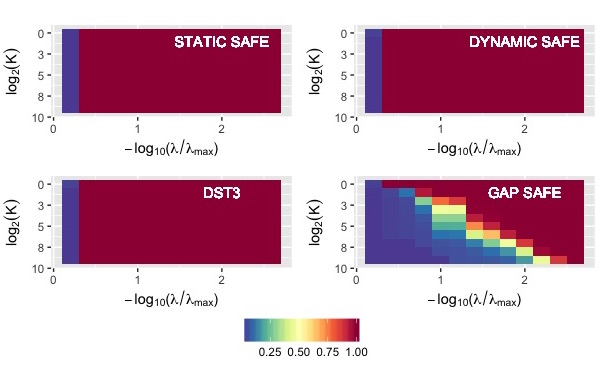
\includegraphics[width=0.8\linewidth]{screening.jpeg}
  \caption{Experiments on a synthetic dataset($\rho = 0.5, \gamma_1 = 10, \gamma_2 = 4, \tau = 0.2$.  Proportion of active variables, \textit{i.e},variables that not safely eliminated, as a function of parameter $\lambda$ and the number of iterations $K$. More blue means more variables eliminated and better screening.}
\end{figure}

I run the ISTA-BA algorithm mentioned in the paper to obtain the sparse-group lasso estimator for a non-decreasing sequence of T regularization parameters $\lambda_t := \lambda_{\text{max}} 10^{-\frac{\delta t}{T-1}}$. By default, we choose $\delta = 3$ and $T = 100$. The weights $w_g = \sqrt{n_g}$.  Here, due to time limit, I only run a couple $\lambda_t$($t \in [1,7,13,19,25,31,37,43,49,55,61,67,73]$), 13 $\lambda_t$ in total,  to illustrate the screening impact. The distance between each $\lambda_t$ is  6, so I  did lose some finer detail compared to the original paper.  Figure 1 shows that \textbf{GAP SAFE} screening rule clearly outperform the other three screening methods.  


\subsection{Time to convergence}
\begin{figure}[h]
  \centering
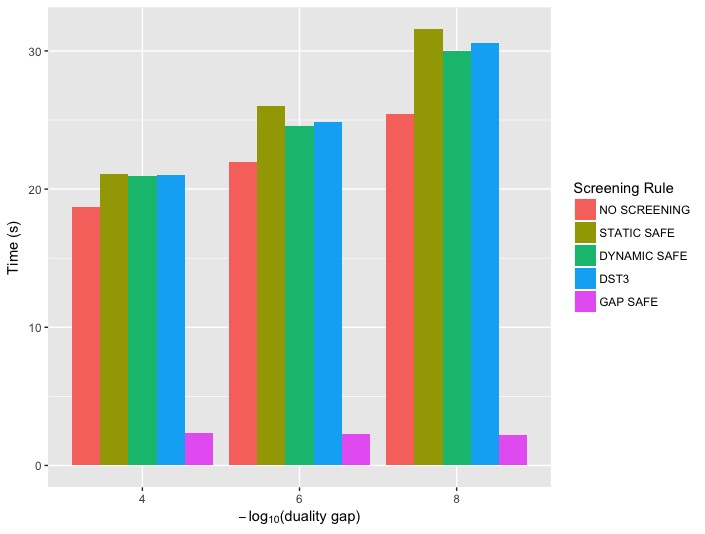
\includegraphics[width=0.8\linewidth]{time.jpeg}
  \caption{Time to reach convergence, w.r.t the accuracy on  the duality gap, using various screening strategies}
\end{figure}

In this experiment, I run the algorithm for a non-decreasing sequence of 10 regularization parameters and record the time it took for all the $\lambda_t$ to reach the duality gap accuracy. There are 10 $\lambda_t$  with ($t \in [1,2,3,4,5,6,7,8,9,10]$).  It seems from Figure 2 that \textbf{GAP SAFE} screening rule is much faster than the rest. This is because that since the $\lambda_t$ is all relatively large, the screening effct of \textbf{GAP SAFE} is obviously significant.  Also it seems that no screening is a bit faster than the rest three screening rules, this is simply due to the inefficiency of my programming..  They should be roughly on the same level [1]. 



\section*{References}


\small


[1]Ndiaye, Eugene, et al. "Gap safe screening rules for sparse-group lasso." (2016) {\it Advances in Neural Information Processing
  Systems}

[2] F. Bach, R. Jenatton, J. Mairal, and G. Obozinski. Convex optimization with sparsity-inducing norms.(2012) {\it Foundations and Trends in Machine learning} 4(1): 1-106

[3] Jenatton, Rodolphe, et al. "Proximal methods for sparse hierarchical dictionary learning."(2010) {\it Proceedings of the 27th international conference on machine learning} (ICML-10).

\end{document}
